\documentclass[border=2pt]{standalone}
% Computer Modern, the font of the handouts (pdflatex)
\usepackage{amsmath}
\usepackage{tikz}
\usepackage{pgfplots}
\pgfplotsset{compat=1.18}
\usetikzlibrary{arrows.meta,calc}
\definecolor{cA}{HTML}{2A78D6}
\definecolor{cB}{HTML}{EB6834}
\definecolor{cC}{HTML}{1BAF7A}
\definecolor{cD}{HTML}{EDA100}
\definecolor{cE}{HTML}{E87BA4}
\definecolor{nodeblue}{HTML}{1565C0}
\definecolor{linkgray}{HTML}{546E7A}
\definecolor{lightgray}{HTML}{CFD8DC}
\definecolor{txt}{HTML}{263238}
\definecolor{band}{HTML}{EEEEEE}
\definecolor{uUnused}{HTML}{BDBDBD}
\definecolor{uLow}{HTML}{2E7D32}
\definecolor{uMid}{HTML}{F9A825}
\definecolor{uHigh}{HTML}{EF6C00}
\definecolor{uFull}{HTML}{C62828}
\definecolor{uOver}{HTML}{7B1FA2}
\tikzset{
  nd/.style={circle, fill=nodeblue, draw=white, line width=0.7pt, minimum size=#1, inner sep=0pt},
  nd/.default=3.2mm,
  nlab/.style={font=\footnotesize\bfseries, text=txt, inner sep=1pt},
  lbl/.style={font=\scriptsize, text=txt, fill=white, fill opacity=0.85, text opacity=1, inner sep=0.7pt},
  arr/.style={-{Stealth[length=1.9mm, width=1.5mm]}},
}
\pgfplotsset{
  lab/.style={
    scale only axis, axis lines*=left, grid=major, grid style={black!12},
    tick label style={font=\small}, label style={font=\normalsize},
    ylabel style={align=center},
    legend style={draw=none, fill=none, font=\small},
    legend cell align=left, tick align=outside, axis line style={black!60},
    every axis plot/.append style={line width=1.1pt},
  },
  % the series differ in color, marker and line style (readable in black and white);
  % the second series has hollow markers, visible where the two curves overlap
  s1/.style={cA, solid, mark=*, mark size=1.7pt},
  s2/.style={cB, densely dashed, mark=square*, mark size=1.6pt, mark options={solid, fill=white}},
  s3/.style={cC, dashdotted, mark=diamond*, mark size=2.1pt, mark options={solid}},
  s4/.style={cD, densely dotted, mark=triangle*, mark size=2.1pt, mark options={solid, fill=white}},
  s5/.style={cE, dashed, mark=triangle*, mark size=2.1pt, mark options={solid, rotate=180}},
  ebars/.style={error bars/.cd, y dir=both, y explicit,
    error bar style={solid, line width=0.9pt}, error mark options={solid, rotate=90, mark size=2.2pt}},
}
\begin{document}
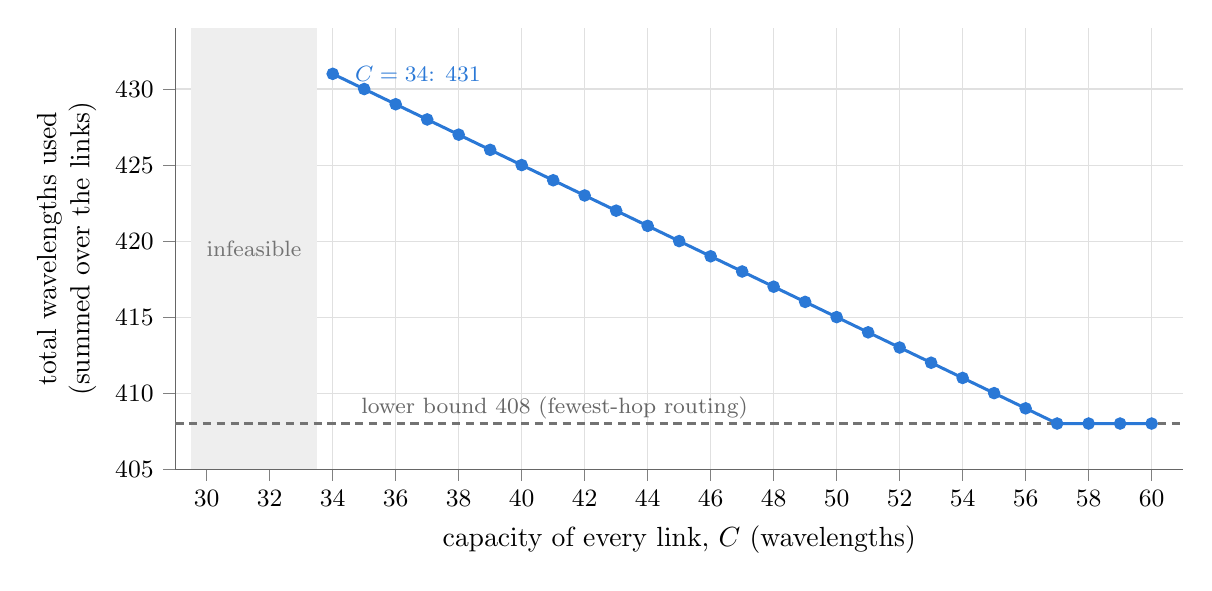
\begin{tikzpicture}\begin{axis}[lab, width=128mm, height=56mm, xmin=29, xmax=61, ymin=405, ymax=434.0, xlabel={capacity of every link, $C$ (wavelengths)}, ylabel={total wavelengths used\\(summed over the links)}]
\fill[band] ({axis cs:29.5,0}|-{rel axis cs:0,0}) rectangle ({axis cs:33.5,0}|-{rel axis cs:0,1});
\node[font=\footnotesize, text=black!55, align=center] at ({axis cs:31.5,0}|-{rel axis cs:0,0.5}) {infeasible};
\draw[black!55, densely dashed, line width=0.8pt] ({rel axis cs:0,0}|-{axis cs:0,408}) -- ({rel axis cs:1,0}|-{axis cs:0,408});
\node[font=\footnotesize, text=black!60, anchor=south west, inner sep=1.5pt] at ({rel axis cs:0.18,0}|-{axis cs:0,408}) {lower bound 408 (fewest-hop routing)};
\addplot[s1] coordinates {(34,431) (35,430) (36,429) (37,428) (38,427) (39,426) (40,425) (41,424) (42,423) (43,422) (44,421) (45,420) (46,419) (47,418) (48,417) (49,416) (50,415) (51,414) (52,413) (53,412) (54,411) (55,410) (56,409) (57,408) (58,408) (59,408) (60,408)};
\node[font=\footnotesize, text=cA, anchor=west] at (axis cs:34.4,431) {$C = 34$: 431};
\end{axis}\end{tikzpicture}
\end{document}
